\subsubsection{Logger}
Struktura:
\begin{itemize}
	\item storage/src/shared/log.erl – moduł
\end{itemize}

Moduł loggera. Wypisuje komunikaty na standardowe wyjście. Węzeł zbudowany w trybie release nie posiada uruchomionej konsoli. Wtedy logi trafiają w domyślne miejsce: log/erlang.log.1

Interfejs loggera przedstawia \autoref{fig:log-module}. Dostępne są trzy funkcje logujące informacje: log:info, log:warn oraz log:error. Pozwalają logować informacje różnych typów. O tym, czy dana funkcja wypisze komunikat na ekran decyduje poziom logowania ustawiony w konfiguracji aplikacji. Szczegóły przedstawia rozdział 3.5 Pliki konfiguracyjne. Możliwe poziomy logowania:
\begin{itemize}
	\item info: wszystkie funkcje wypisują komunkaty. Z użyciem tej funkcji wypisywane są informacje o zdarzeniach aktualnie zachodzących w systemie.
	\item warn: wywołania log:info są ignorowane. . Przy użyciu tej funkcji wypisywane są przykładowo informacje o niepoprawnej sumie kontrolnej
	\item error: wywołania log:info oraz log:warn są ignorowane. Zarezerwowana jest dla krytycznych błędów.
	\item none: wszystkie funkcje są ignorowane, nic nie jest wypisywane
\end{itemize}

Interfejs tych trzech funkcji jest identyczny. Każa występuje w dwóch wersjach:
\begin{itemize}
	\item log:xxxx(Message) – wypisuje wiadomość (typu string())
	\item log:xxxx(Format, [Args]) – wypisuje sformatowany napis (string()) z wstawionymi argumentami. Obowiązuje standardowe formatowanie jak we wbudowanym module io.
\end{itemize}

\begin{figure}[!htbp]
	\centering
	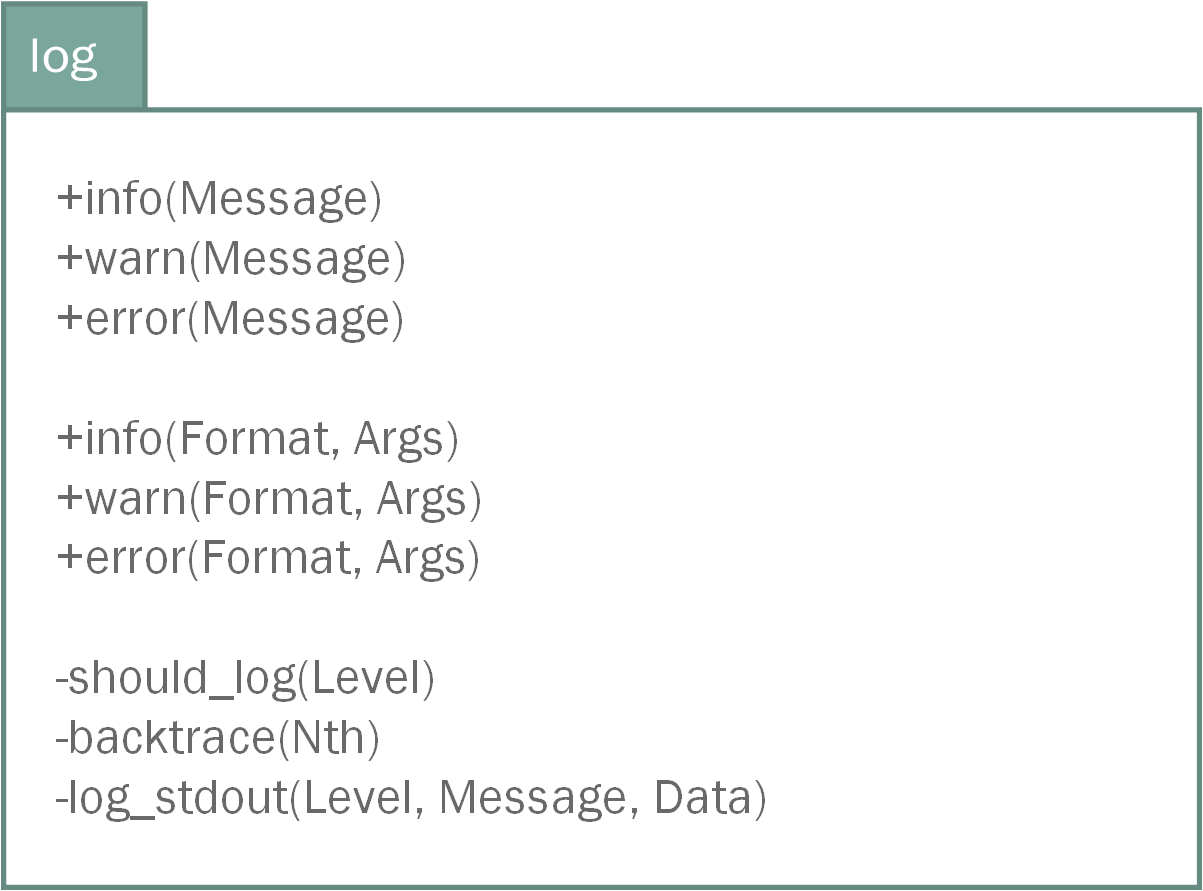
\includegraphics[width=0.7\textwidth]{log-module}
	\caption{Struktura modułu loggera.}
	\label{fig:log-module}
\end{figure}

Wypisany komunikat ma strukturę:

\centerline{\texttt{[level] HH:MM:SS (module:function/arity): message}}

Przykładowo:
\begin{lstlisting}
[info] 18:51:33 (storage_dist_srv:handle_cast/2):
			'ds3@michal-pc' has joined the cluster!
\end{lstlisting}

Określenie lokalizacji (funkcji, z której nastąpiło logowanie) odbywa się automatycznie, poprzez symulowane rzucenie wyjątku, złapanie go, a następnie zbadanie stosu wywołań. Może do negatywnie wpływać na wydajność. Logowanie można więc całkowicie zablokować odpowiednią opcją kompilacji.
